\documentclass{article}

\usepackage{graphicx}

\title{Test Bench Manual}
\author{Boris Korzh}
\date{29th October 2012}
\begin{document}
\maketitle
\begin{center}
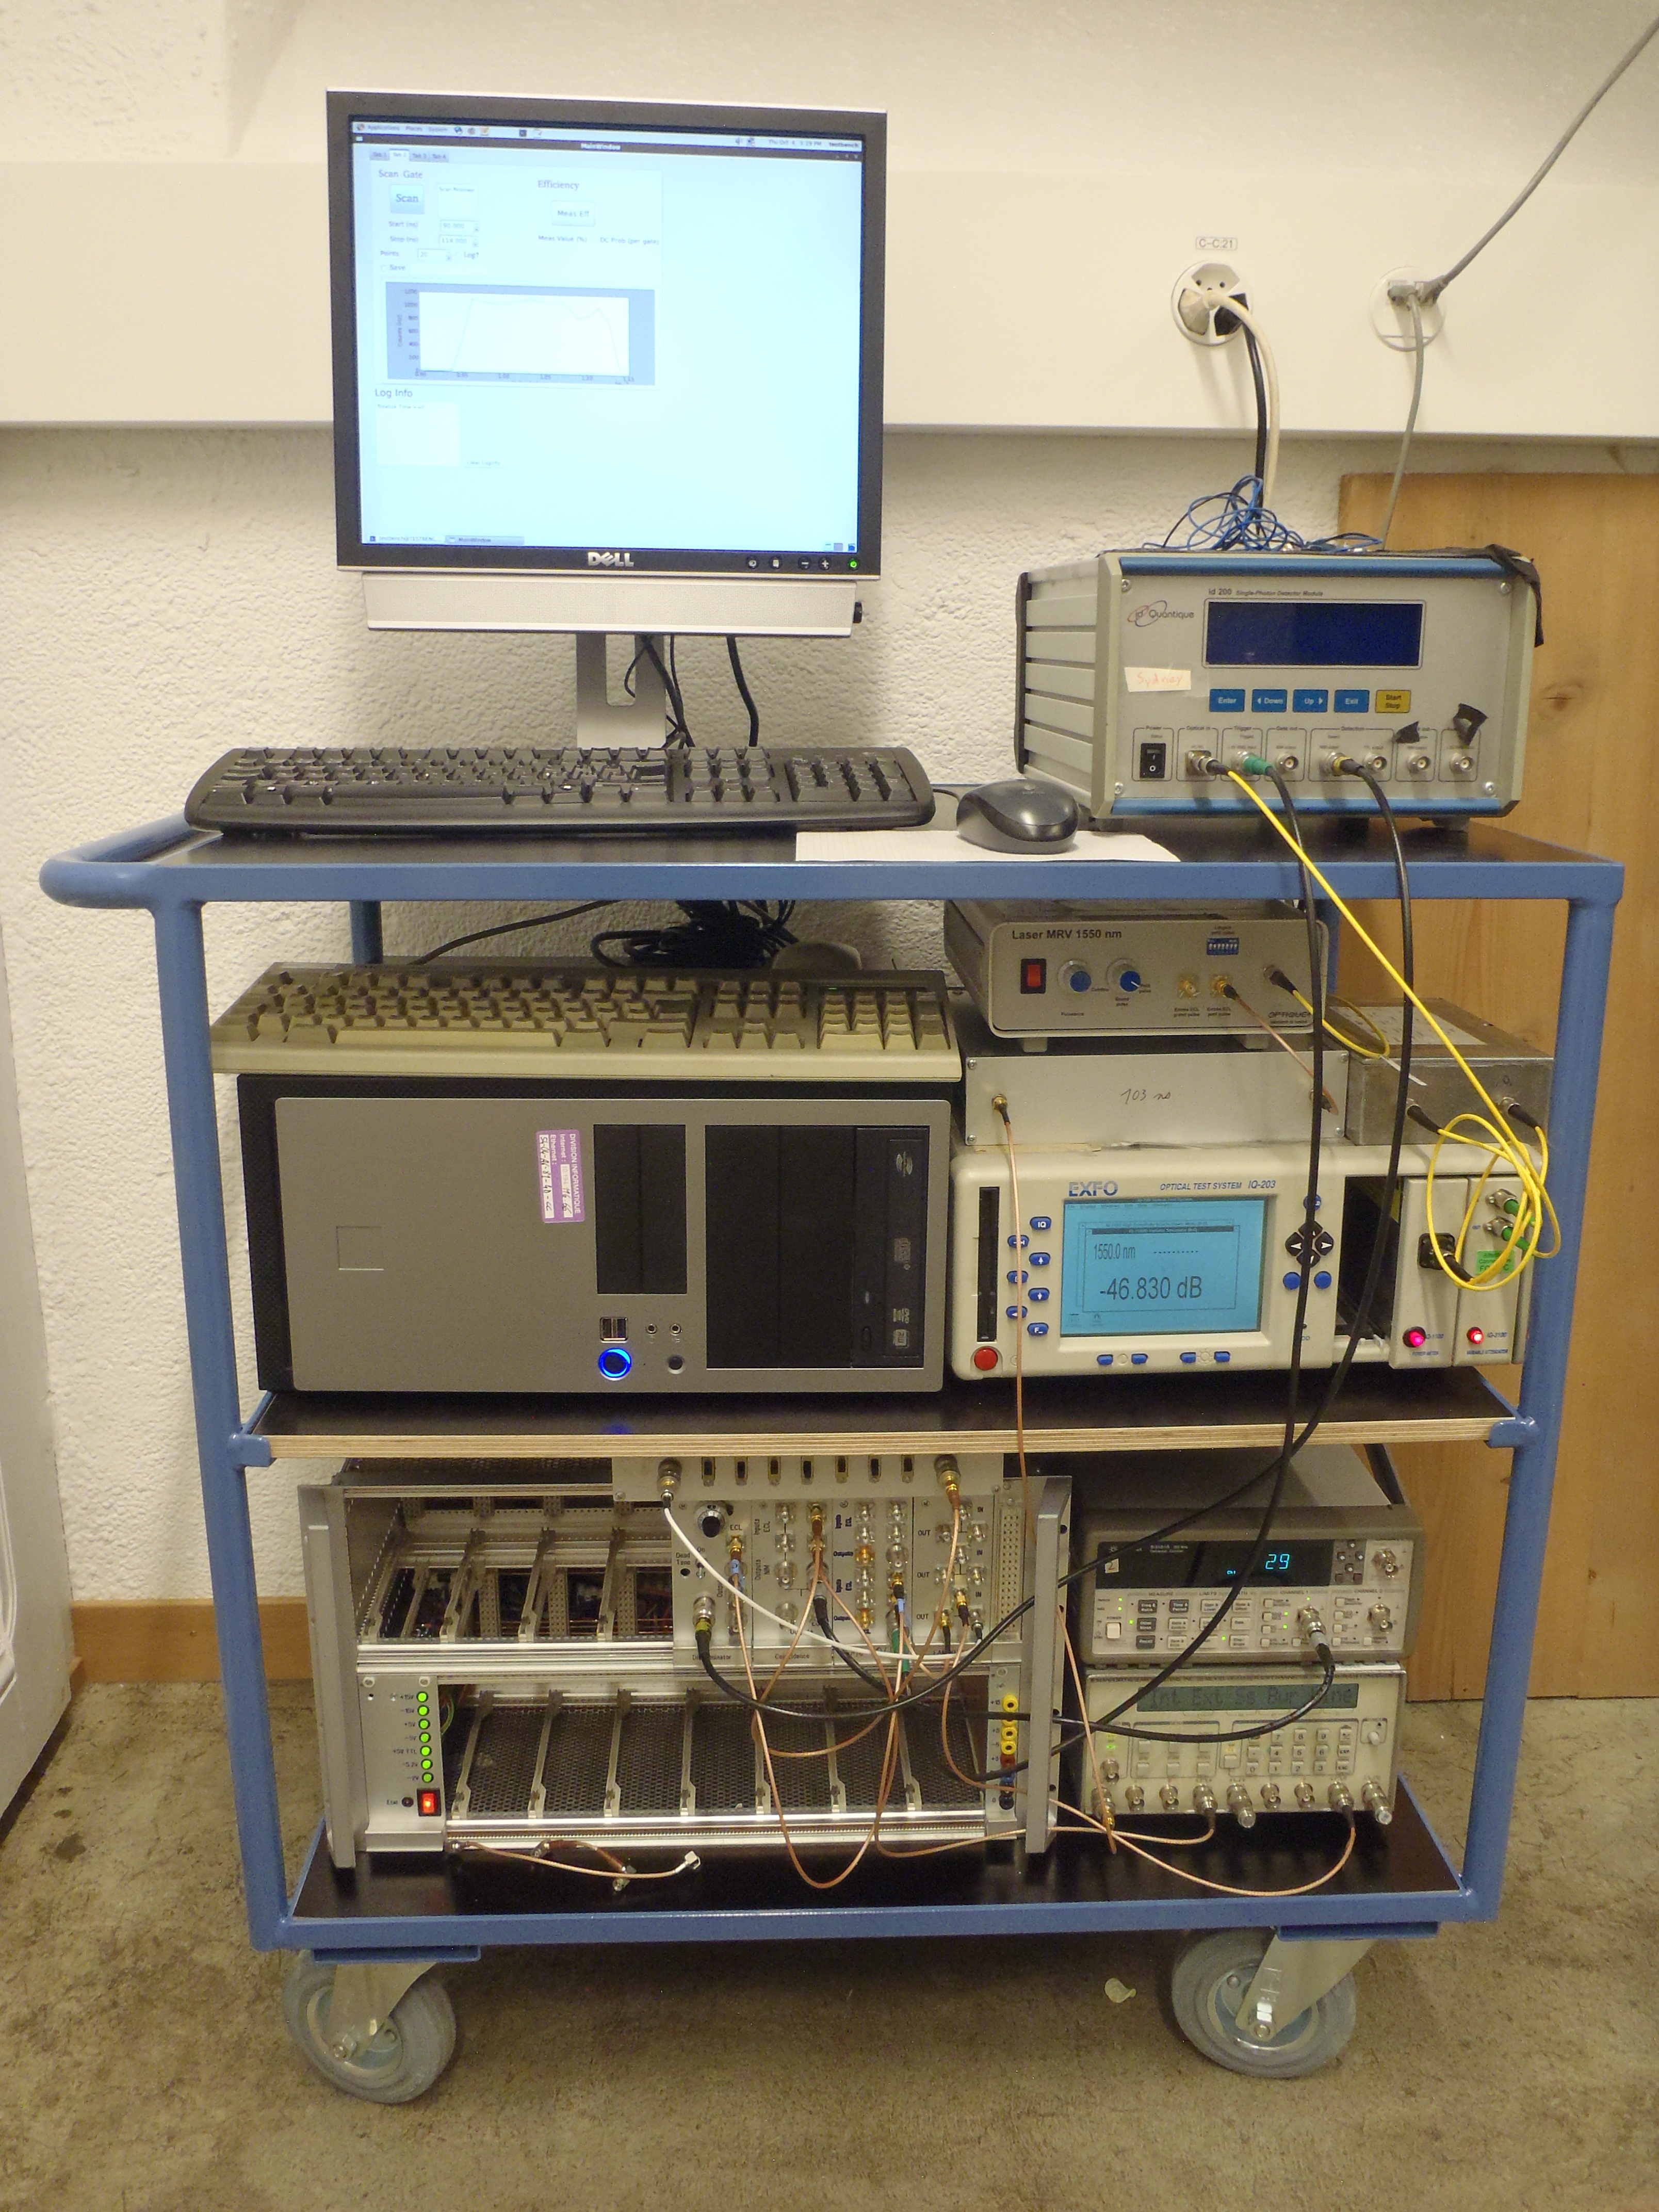
\includegraphics[width=10cm]{images/testbench1.JPG}
\end{center}
% == Specs


\section{Specifications}
\begin{center}
\begin{tabular}{ | l | l |  }
\hline
\emph{Parameter} & \emph{Value} \\ \hline
{\bf General } &   \\ \hline
Detector Type & Gated Mode Detectors \\ \hline
Detector Trigger Input & TTL, NIM, ECL \\ \hline

{\bf Pulse Generator } &   \\ \hline
Maximum Frequency & 1 MHz  \\ \hline
Maximum Delay & 1000 sec  \\ \hline
Resolution & 5 ps  \\ \hline
Accuracy & 1500 ps  \\ \hline

\bf{Laser} & \\ \hline
Wavelength & 1550 nm \\ \hline
Pulse Width (FWHM) & 490 ps \\ \hline
\bf{Counter} & \\ \hline

Signal Input & TTL, NIM, ECL \\ \hline
\end{tabular}
\end{center}
% == Setup


\section{Setup}

\begin{figure}
\centering
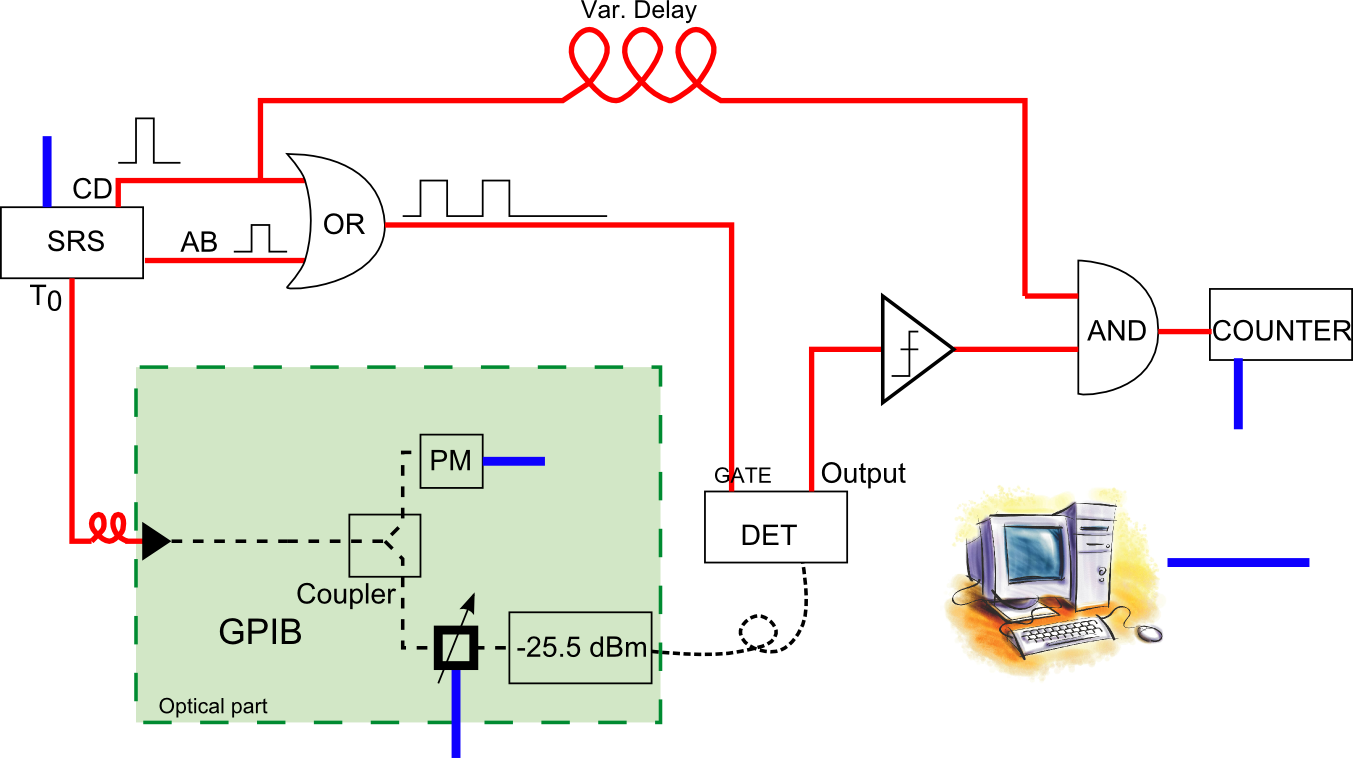
\includegraphics[width=12cm]{images/SetupGated2.png}
\caption{Setup of test bench.}
\label{setup}
\end{figure}
The test bench setup is shown in Figure~\ref{setup}. The whole system is synchronized from the Pulse Generator (SRS). This generates trigger pulses which control all of the instruments. The optical part of the system is triggered by the $T_{0}$ signal which activates the pulsed laser source. The optical signal is split at a coupler with one part going to a power meter, whilst the other is attenuated accordingly with a variable and a fixed attenuator, to achieve the required number of photons per pulse. The variable attenuator also has a shutter which is activated during dark count characterization.

During efficiency characterization and scanning of the gate shape, only the CD signal triggers the detector gate, the $AB$ signal is set to zero. The delay between the $T_0$ and $CD$ pulses must be synchronized such that the light pulse coincides with the correct point of the detector gate. The detector output is then counted with an external counter, as a coincidence with a delayed $CD$ pulse. 

Afterpulse characterization uses the double window method, hence both the $AB$ and $CD$ signals are used to trigger the detector. The laser pulse in this case is synchronized with the gate generated due to the $AB$ pulse, whilst no light is sent onto the detector during the $CD$ gate. Only the detections generated during the $CD$ gate are registered by the external counter, hence by varying the delay between $AB$ and $CD$ it is possible to evaluate the afterpulse probability as a function of deadtime. In order to ensure that there is a detection in every $AB$ window, the average photon number of photons per pulse is increased, to cause saturation.  

% === Software

\section{Software}

The main test bench control software has a Python user interface and comprises of 4 tabs, which are illustrated in Figures \ref{tab1}, \ref{tab2}, \ref{tab3} and \ref{tab4}. 

\begin{figure}
\centering
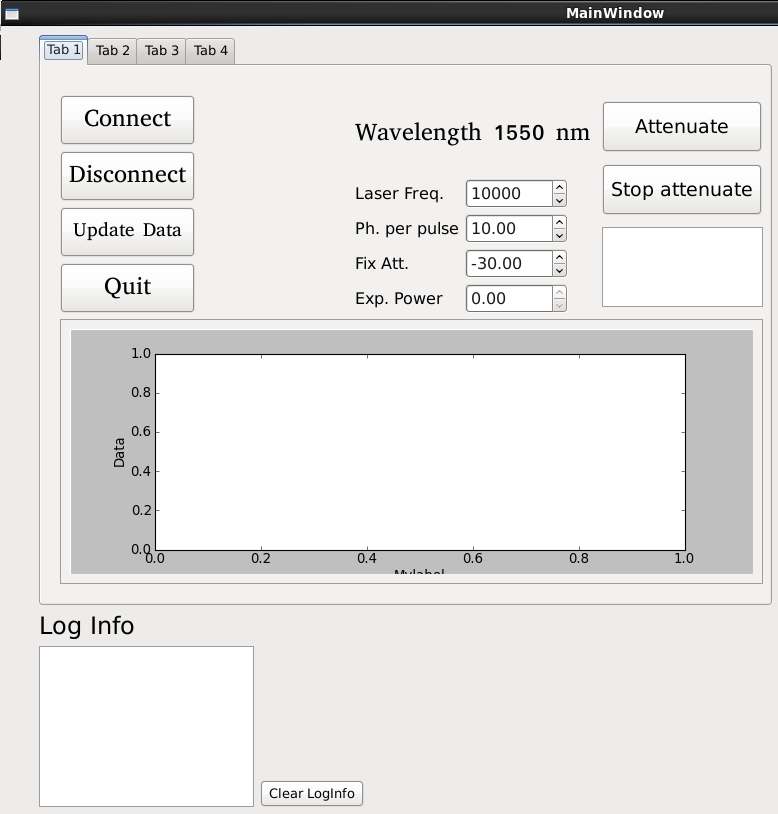
\includegraphics[width=7.8cm]{images/tab1.png}
\caption{Tab 1 of main control program. Optical pulse attenuation settings.}
\label{tab1}
\end{figure}

\begin{figure}
\centering
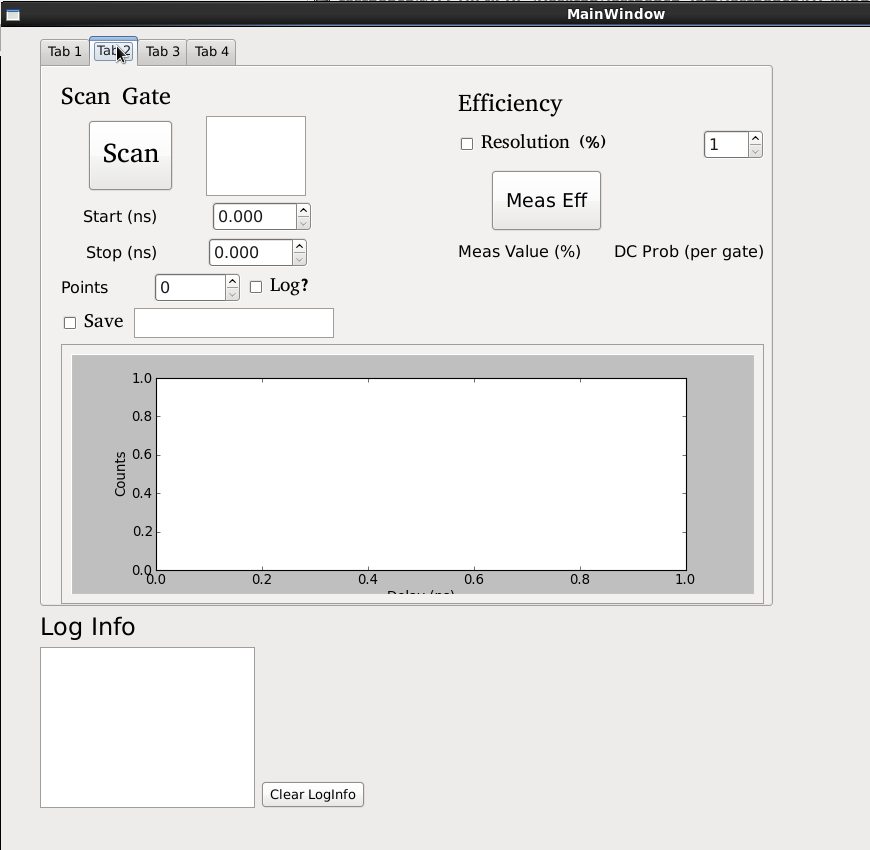
\includegraphics[width=7.8cm]{images/tab2.png}
\caption{Tab 2 of main control program. Detector efficiency, dark count and scan of the gate characterization, settings and results.}
\label{tab2}
\end{figure}

\begin{figure}
\centering
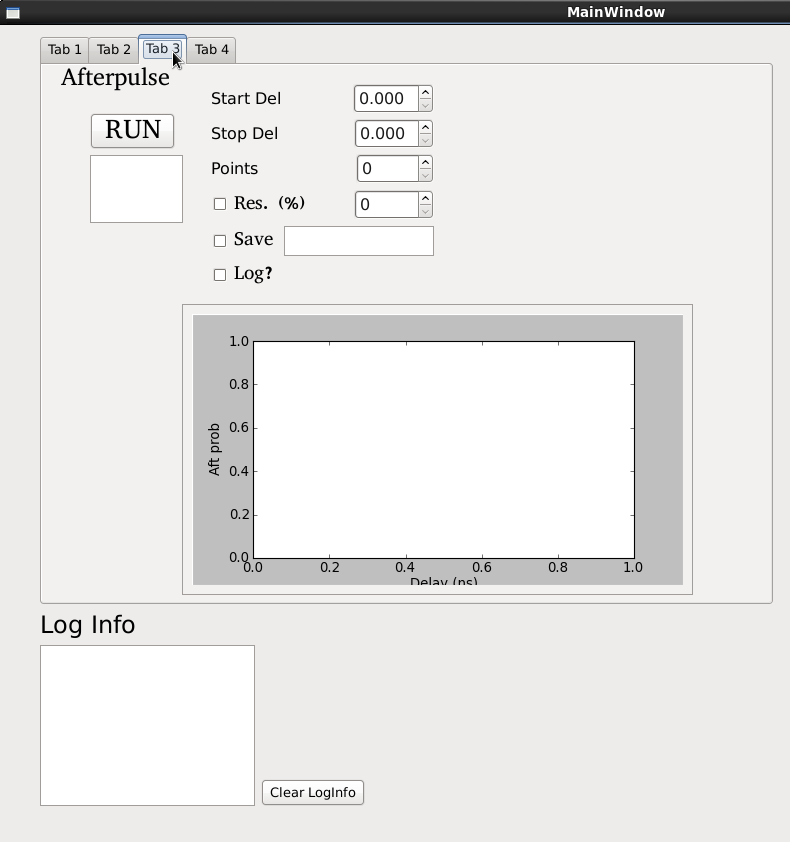
\includegraphics[width=7.8cm]{images/tab3.png}
\caption{Tab 3 of main control program. Afterpulse characterization settings and results.}
\label{tab3}
\end{figure}

\begin{figure}
\centering
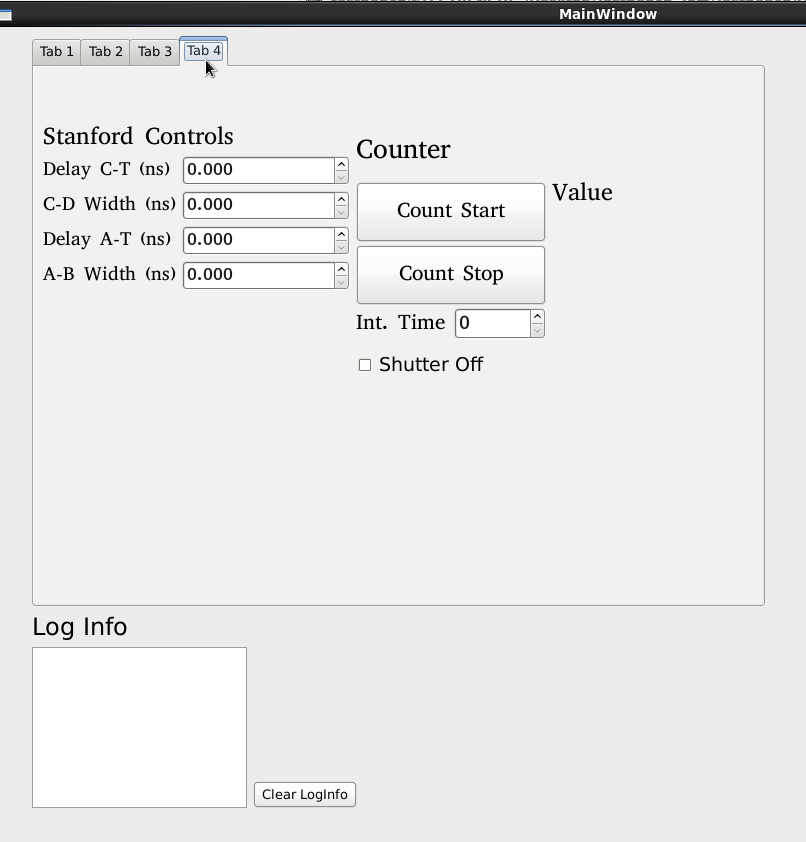
\includegraphics[width=7.8cm]{images/tab4.png}
\caption{Tab 4 of main control program. Pulse generator settings and realtime external counter display.}
\label{tab4}
\end{figure}

% ==== Initialisation 

\section{Initialization}
This section describes the procedure for the initialization of all of the test bench components. When characterizing a detector, it is preferable to carry out the tests in the order that they appear in this manual, since some of the values obtained in a given section are often required at a later stage for a different parameter characterization.

% == External Components

\subsection{External Components}

\begin{itemize}

\item
Connect the output of the OR Port (Porte/OU) on the Electronic circuit rack to the external trigger input on the detector to be tested, using either the ECL or NIM signal appropriately, depending on the detector requirements.

\item
Connect the detector output to the Discriminator Analog Input on the Electronic circuit rack.

\item
Connect the output of the optical attenuator to the detector optical input. 

\item
Power ON all of the remaining components in the following order:

\begin{itemize}
\item{Detector to be tested}
\item{Power meter/Attenuator}
\item{Laser}
\item{SRS Pulse Generator}
\item{Agilent Counter}
\item{Electronic component rack}
\end{itemize}

\item
After the initial loading, the Power Meter/Attenuator meter display will remain in the terminal command view. Use it's dedicated keyboard (EXFO PMD Keyboard) to to enter:

\begin{itemize}

\item
Command: \emph{win}
\end{itemize}
The windows display should now load on the screen. 

\end{itemize}

% == PC and Software

\subsection{PC and Software}

\begin{itemize}
\item
Turn on the PC and log on. 
\begin{itemize}
\item
Username = TESTBENCH
\item
Password = tb
\end{itemize}

\item
Open the {Terminal}
\begin{itemize}
\item 
\emph{Applications $>$ System Tools $>$ Terminal}
\end{itemize}

\item
Change to correct directory:
\begin{itemize}
\item
Command: \emph{cd Desktop/Testbench\_Prog}
\end{itemize}

\item
View files in directory:
\begin{itemize}
\item
Command: \emph{ls}
\end{itemize}

\item
Select the latest version of the program and run it (xxxx\_xx\_xx corresponds to the program modification date):
\begin{itemize}
\item
Command: \emph{python run\_main\_xxxx\_xx\_xx}
\end{itemize}

\end{itemize}





% section for software initialisation instructions

The following describes the initialization of the user interface software.

\begin{itemize}

\item
Select path for attenuation log file. In Main Window:
\begin{itemize}
\item
Press: \emph{Tab 1 $>$ Connect}
\item 
Select \emph{Data} folder and confirm
\end{itemize}

\label{sec:soft_init}

\item
Set the attenuator parameters. Remain in \emph{Tab 1} (default values):
\begin{itemize}
\item
\emph{Laser Freq.}: 10,000
\item
\emph{Ph. per pulse}: 1 (for Efficiency, Dark Count and Gate Shape measurements) or 50 (for Afterpulsing characterization). 
\item
\emph{Fix Att.}: -25.50
\end{itemize}
\item
Press \emph{Attenuate}. The expected optical power value will be calculated and the attenuation procedure will begin. Optical power measurements will be logged in the graph. Wait until the power is stabilized (at least 5 consecutive points within a 0.05 dBm range).
\item
If any of the attenuator values need to be changed, \emph{Stop attenuate} must first be pressed. 

\end{itemize}

%  Manual delay adjustment
\subsection{Circuit Delay Synchronization}

\begin{figure}
\centering
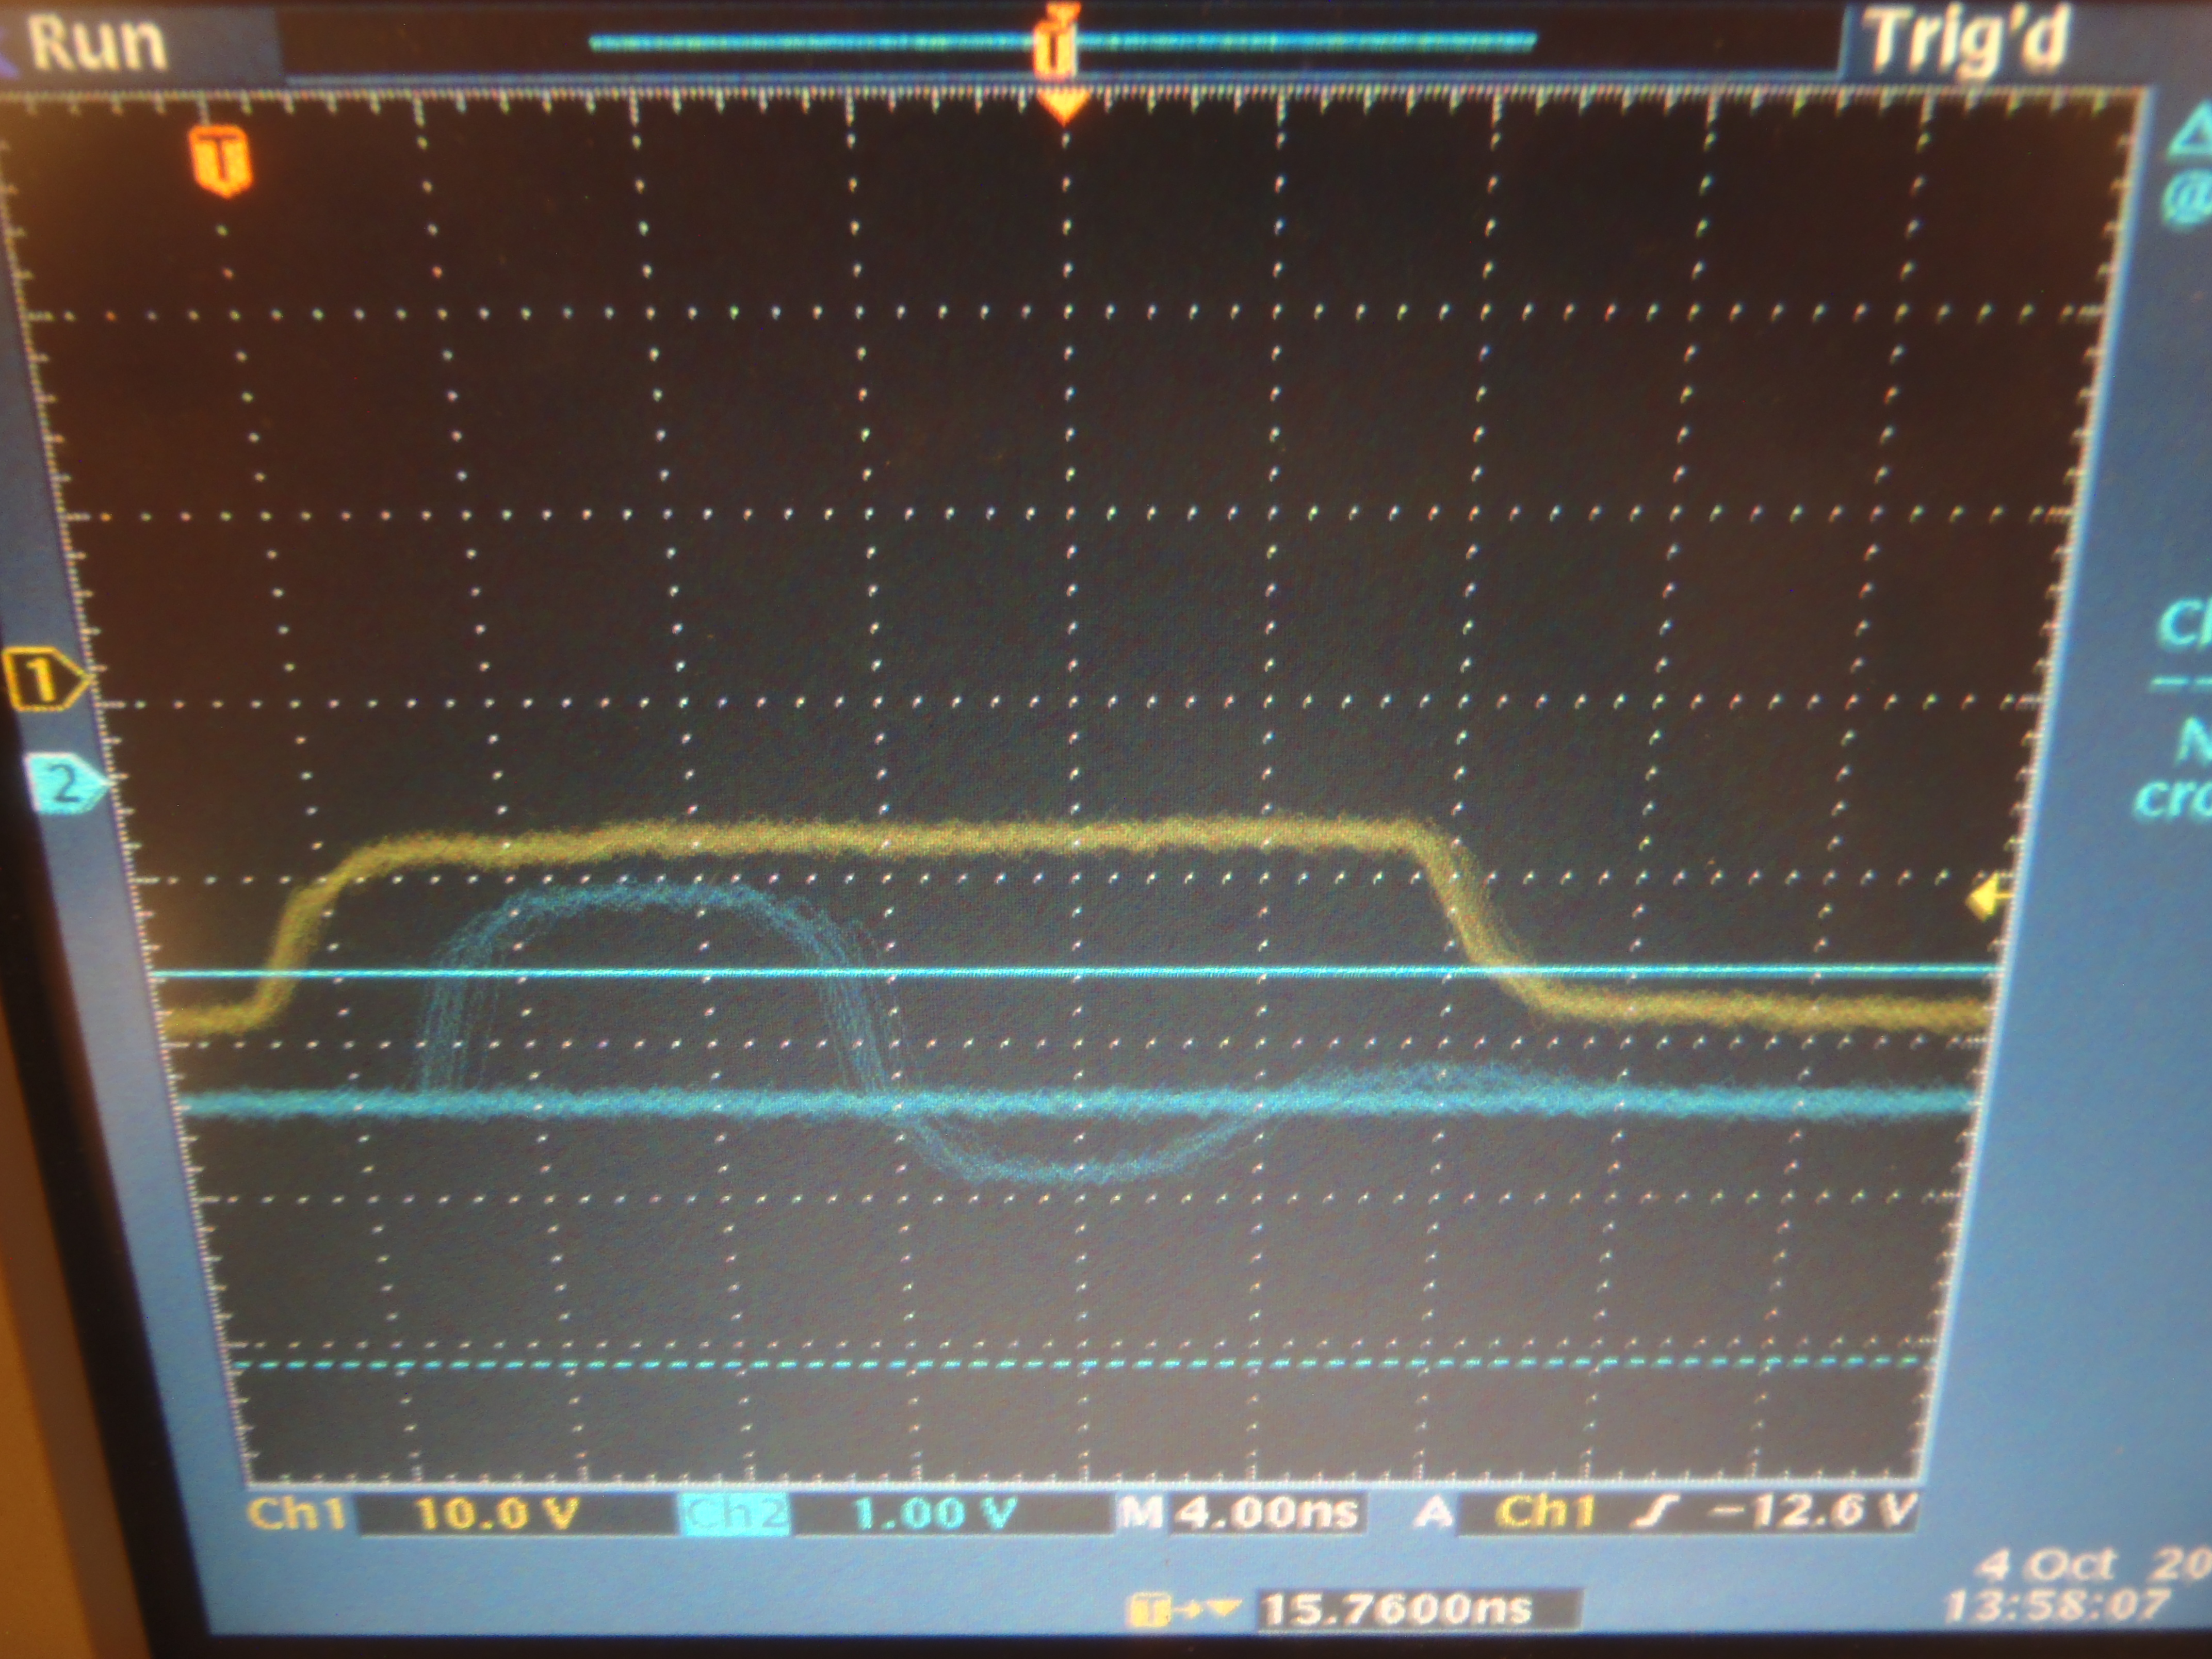
\includegraphics[width=10cm]{images/trace.JPG}
\caption{$CD$ signal (yellow) and the detector output pulse (blue) viewed on an oscilloscope, showing the correct synchronization just before the coincidence port. Here the detector gate duration was 20 ns.}
\label{trace}
\end{figure}

This section deals with the unknown internal delay of the detector to be tested. In order to obtain meaningful results from the test bench it is important to match the unknown delay of the detector with the external manual delay on the test bench. The aim is have the detector output pulse rising edge within the CD pulse created by the SRS Pulse Generator. This will ensure that all of the detection counts are counted by the test bench. The easiest way to achieve this is to use an \emph{Oscilloscope}, which is not necessarily stored on the test bench at all times.

\begin{itemize}
\item
Disconnect the two inputs of the \emph{Coincidence Port} on the Electronic circuit rack, one coming from the \emph{Discriminator} and one from the \emph{Manual Delay} module. 

\item
View the signals on the oscilloscope. Set the trigger on the CD pulse (coming from the manual delay).
\begin{itemize}
\item
\emph{Important}: Use offset blocks on both inputs of the Oscilloscope, biased at -5.2 V. This is due to the fact that the signals involved are ECL, which might not be within the range of the Oscilloscope.
\end{itemize}

\item 
In \emph{Tab 4}, complete the Stanford Controls (Pulse Generator) settings. 
\begin{itemize}
\item
\emph{Delay C-T}: 100 ns (arbitrary for the moment)
\item
\emph{C-D Width}: Set this to 5 ns {\bf longer} than the gate time of the detector e.g. 25 ns for a detector with a gate duration setting of 20 ns.
\item
\emph{Delay A-T}: 0 ns
\item
\emph{A-B Width}: 0 ns
\end{itemize}

\item
The CD pulse should now be visible on the Oscilloscope. The detector output pulse may or may not be visible.
\item
Increase the Discriminator level until the detector output signal disappears, then decrease it by approximately 1.00 division beyond the level at which pulses appear.
\item
At the moment it is unlikely that the laser pulse is synchronized with the detector gate time. Hence the detection pulses visible are due to dark-counts.  In order to find the ``light'':
\begin{itemize}
\item
You should look at the detection frequency, this could either be displayed on the detector itself, or you can use the frequency read out on the oscilloscope.
\item
Increase the \emph{Delay C-T} by 1 ns at a time (80ns is a good starting point) until the detection rate increases. This should also correspond to a more defined line on the oscilloscope.
\item
Keep increasing the delay until the detection rate drops off once more, but note what was the highest detection rate achievable. 
\item
Now decrease the delay once more in order to set the {\bf maximum} possible delay whilst having a detection rate value close to the highest achieved. This corresponds to the laser pulse coinciding with the start of the detector gate. 
\end{itemize}

\item
Some detector pulses may occur at a later time, this is normal since a dark detection may occur at different times during the gate.
\item
At this point, the main detector pulse might not be within the CD pulse. They should be synchronized with each other. Change the Manual Delay settings so that the CD pulse begins at least 1 ns before the earliest rising edge of the detector output pulse. The traces should look as per Figure \ref{trace}.
\begin{itemize}
\item
\emph{Important}: Disconnect the CD line (Manual Delay) from the Oscilloscope, before changing the delay. Signal spikes from the module during switching may damage the Oscilloscope. 
\end{itemize}

\item
The latest occurring rising edges of the detector output should be within the CD pulse. If not, adjust the \emph{C-D Width} value accordingly. This will ensure that all of the detections within the detector gate are recorded by the test bench.

\item
Once the delays are synchronized, reconnect the two signal lines to the Coincidence Port on the Electronic Circuit rack.

\item
In MainWindow, \emph{Tab 4}, select an \emph{Integration Time} of 1 second and press \emph{Count Start}.

\item 
A count rate value should appear in the bottom right of the display. This value should be approximately equal to the count rate value on the detector display (if available). This indicates that the test bench is set up correctly. 



\end{itemize} 
 
 % end of initialization
 
\section{Characterization Tests}

\subsection{Scan of the Gate}

% ==== Scan the gate section

It is now possible to perform a scan of the gate. Doing this before measuring the detector efficiency is important in order to select the desired point on the gate (typically the middle) for the measurement.

\begin{itemize}
\item
In \emph{Tab 4}, select the integration time for each measurement (units of seconds). 1 second is sufficient for the initial scan of the gate.
\item
Select \emph{Tab 2}. Complete the Scan Gate parameters:
\begin{itemize}
\item
\emph{Start}: This should be in the region of the value of Delay C-T minus the C-D Width as set up in the previous section.
\item
\emph{End}: This should be higher than the Delay C-T set in the previous section.
\item
\emph{Points}: As required.
\end{itemize}

\item
It is possible to save the data by selecting the \emph{Save} option and designating a file name. The file destination will be the \emph{Data} folder as selected during the Connection procedure as described in Section \ref{sec:soft_init}.
\item
The gate scan will appear in the Main Window. Note that the scan is reversed in time in relation to the delay, hence the beginning of the gate corresponds to the longer delay values.
\end{itemize}


%%% Efficiency Measurement

\subsection{Detector Efficiency}
\label{sec:eff}
It is possible to carry out a measurement of the detector efficiency at a determined position on the gate.
\begin{itemize}
\item
In \emph{Tab 4} select the required position on the gate with the \emph{Delay C-T} value.
\item 
Select the required \emph{Integration Time}.
\item
In \emph{Tab 2}, press \emph{Meas Eff}. The resulting Efficiency and Dark Count Probability per gate will be calculated. 

\end{itemize}


%%% Afterpulse Measurements

\subsection{Afterpulse probability}

In order to characterize the Afterpulse performance of the detector it is necessary to increase the optical power incident on the detector, in order to saturate detections to one every gate. The test bench uses the double window method for measuring the afterpulse probability.

\begin{itemize}
\item
In \emph{Tab 1} increase the number of photon number.
\begin{itemize}
\item
Press: \emph{Stop Attenuate}.
\item
Increase \emph{Ph. per pulse} to 50.
\item
Press: \emph{Attenuate}.
\item
Wait for the optical power to stabilize.
\end{itemize}

\item
In \emph{Tab 4}:
\begin{itemize}
\item
Copy the \emph{Delay C-T} value to \emph{Delay A-T} field. This should be the value used during the efficiency measurement (Section \ref{sec:eff}), corresponding to the middle of the gate (or the optimum selected position).
\item
Copy the \emph{C-D Width} value to \emph{A-B Width} field, from Section \ref{sec:eff}. 
\end{itemize}

\item
In \emph{Tab 3}, select the desired \emph{Start}, \emph{Stop} times and the number of \emph{Points} for the afterpulsing scan.
\item
Press \emph{Run} to begin the scan. The result will be displayed on the screen. 
\item
The data can be saved using the \emph{Save} option.

\end{itemize}




\end{document}
 